\title{Лекция 11\\Базовый язык программирования для обработки баз знаний}
\author[]{Шункевич Д.В.}
\institute[]{Белорусский государственный университет информатики и радиоэлектроники}

\begin{frame}
	\titlepage
\end{frame}

\begin{frame}{\\Содержание лекции}
	\topline
	\justifying
	Базовые принципы обработки знаний. 1-2-3-элементные конструкции. Произвольные конструкции, поиск и генерация по образцу. Основные положения языка SCP. Понятие scp-программы, scp-процесса, scp-оператора. Понятие scp-операнда, классификация scp-операндов, scp-переменная, scp-константа. Классификация scp-операторов. Организация условных и безусловных переходов, циклов. Реализация подпрограмм. Агентная scp-программа.
	
\end{frame}

\begin{frame}{\\Понятие языка scp}%понятие scp-языка
	\topline
	\justifying
	\vspace{1.5em}
	\begin{SCn}
		\scnheader{Язык SCP}
		\scnidtftext{часто используемый sc-идентификатор}{scp-программа}
	\end{SCn}
		\scntext{пояснение}{В качестве базового языка для описания программ обработки текстов
			\textit{SC-кода} предлагается \textit{Язык SCP}.
			
			\textit{Язык SCP} -- это графовый язык процедурного программирования,
			предназначенный для эффективной обработки \textit{sc-текстов}. \textit{Язык SCP} является языком параллельного асинхронного программирования.
			
			Языком представления данных для текстов \textit{Языка SCP}
			(\textit{scp-программ}) является \textit{SC-код} и, соответственно, любые
			варианты его внешнего представления. 
			
			\textit{Язык SCP} рассматривается как ассемблер для семантического компьютера.}
		\end{frame}

\begin{frame}{sc-код}%sc-код
	содержимое...
\end{frame}
	
\begin{frame}{\\Абстрактная scp-машина}%абстрактная scp-машина
		\topline
		\justifying
		\begin{SCn}
			\scnheader{Абстрактная scp-машина}
			\scniselement{scp-машина}\scnrelto{обобщенная модель}{scp-интерпретатор
			}
		\end{SCn}
			\scntext{примечание}{\textit{Абстрактная scp-машина} представляет собой интерпретатор \textit{scp-программ}, который должен являться частью \textit{платформы интерпретации sc-моделей компьютерных систем} (хотя в общем случае могут существовать варианты платформы, не содержащие такого интерпретатора, что, однако, не позволит использовать достоинства предлагаемой базовой модели}
	\end{frame}

\begin{frame}{\\структура}
	\topline
	\justifying
	\begin{SCn}
	\scnheader{структура}
	\begin{scnrelfromset}{разбиение}
	\scnitem{sc-конструкция нестандартного вида}
	\scnitem{sc-конструкция стандартного вида}
	\begin{scnrelfromset}{разбиение}
		\scnitem{одноэлементная sc-конструкция}
		\scnitem{трехэлементная sc-конструкция}
		\scnitem{пятиэлементная sc-конструкция}
	\end{scnrelfromset}	
	\end{scnrelfromset}
	\end{SCn}
\end{frame}

\begin{frame}{\\sc-конструкция нестандартного вида}
	\topline
	\justifying
	\begin{SCn}
		\scnheader{sc-конструкция нестандартного вида}
		\scntext{пояснение}{Каждая \textit{sc-конструкция нестандартного вида} состоит из произвольного количества \textit{sc-элементов} произвольного типа.}
		\scnrelfrom{пример}{
			\begin{center}
				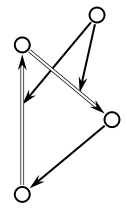
\includegraphics[width=18mm]{figures/sd_sets/pic_ps1.png}
		\end{center}}
	\end{SCn}
\end{frame}

\begin{frame}{\\sc-конструкция стандартного вида}
	\topline
	\justifying
	\begin{SCn}
		\scnheader{sc-конструкция стандартного вида}
		\scntext{пояснение}{В свою очередь, каждый элемент \textit{\mbox{sc-конструкции} стандартного вида} имеет свою условную строго фиксированную позицию в рамках этой \mbox{sc-конструкции} (первый элемент, второй элемент и т. д.). В зависимости от указанной позиции вводятся дополнительные ограничения на тип соответствующего \textit{sc-элемента}.}
	\end{SCn}
\end{frame}

\begin{frame}{\\одноэлементная sc-конструкция}
	\topline
	\justifying
	\begin{SCn}
		\scnheader{одноэлементная sc-конструкция}
		\scntext{пояснение}{Каждая \textit{одноэлементная sc-конструкция} состоит из одного \newline \textit{sc-элемента} произвольного типа.}
		\scnrelfrom{пример}{
			\begin{center}
				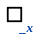
\includegraphics[width=17mm]{figures/sd_sets/pic_ps2.png}
		\end{center}}
	\end{SCn}
\end{frame}

\begin{frame}{\\трёхэлемениная sc-конструкция}
	\topline
	\justifying
	\begin{SCn}
		\scnheader{трехэлементная sc-конструкция}
		\scntext{пояснение}{Каждая \textit{трехэлементная sc-конструкция} состоит из трех \newline \textit{sc-элементов}. Второй элемент всегда является \textit{sc-коннектором}, остальные элементы могут быть произвольного типа.}
		\scnrelfrom{пример}{
			\begin{center}
				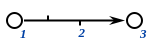
\includegraphics[width=35mm]{figures/sd_sets/pic_ps3.png}
		\end{center}}
	\end{SCn}
\end{frame}

\begin{frame}{\\пятиэлементная sc-конструкция}
	\topline
	\justifying
	\begin{SCn}
		\scnheader{пятиэлементная sc-конструкция}
		\scntext{пояснение}{Каждая \textit{пятиэлементная sc-конструкция} состоит из пяти \newline \textit{sc-элементов}. Второй и четвертый элементы обязательно являются \textit{sc-коннекторами}, остальные элементы могут быть произвольного типа.}
		\scnrelfrom{пример}{
			\begin{center}
				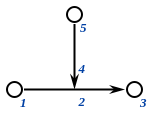
\includegraphics[width=35mm]{figures/sd_sets/pic_ps4.png}
		\end{center}}
	\end{SCn}
\end{frame}


\begin{frame}{\\scp-программа}%scp-программа
	\topline
	\justifying
	\begin{SCn}
		\scnheader{scp-программа}
		\scnsubset{программа в sc-памяти}
		\scnsuperset{агентная scp-программа}
		\end{SCn}
\scntext{пояснение}{Каждая \textbf{\textit{scp-программа}} представляет собой \textit{обобщенную структуру}, описывающую один из вариантов декомпозиции действий некоторого класса, выполняемых в sc-памяти. Знак \textit{sc-переменной}, соответствующей конкретному декомпозируемому действию является в рамках \textbf{\textit{scp-программы}} \textit{ключевым sc-элементом\scnrolesign}.
	
	По сути каждая \textbf{\textit{scp-программа}} представляет собой описание последовательности элементарных операций, которые необходимо выполнить над семантической сетью, чтобы выполнить более сложное действие некоторого класса.}
\end{frame}

\begin{frame}%пример программы
	\scntext{описание примера}{
	\begin{center}
	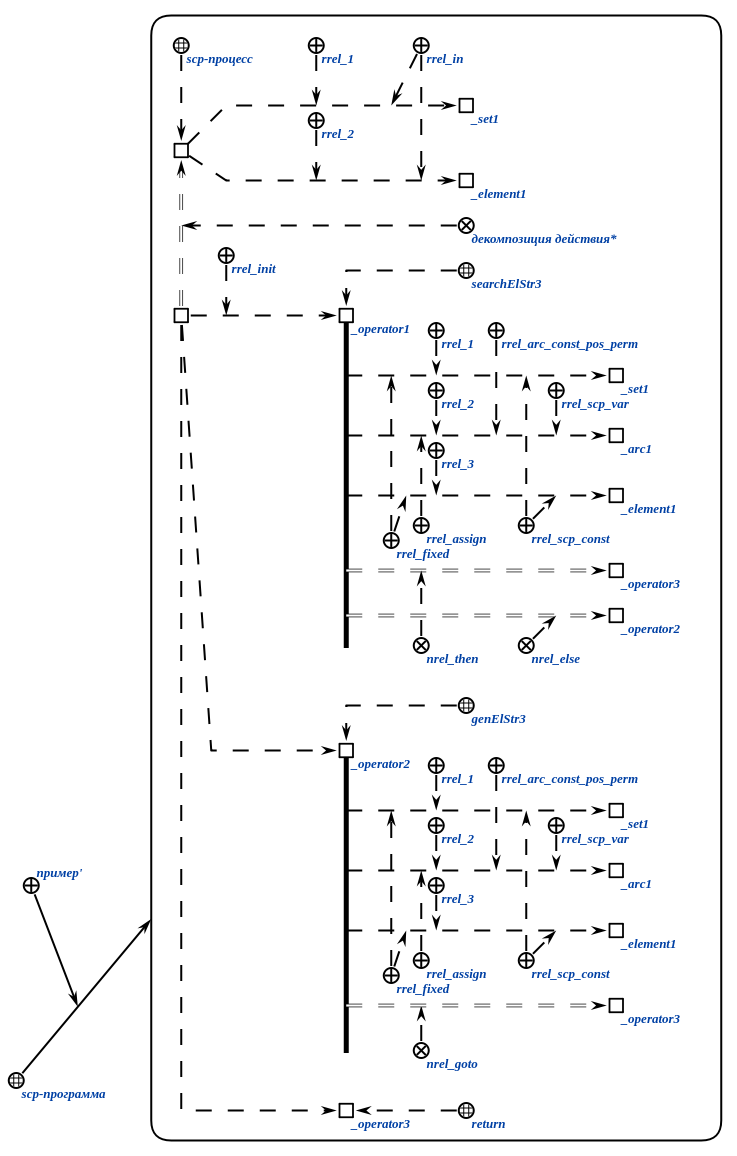
\includegraphics[width=50mm]{figures/sd_sets/program_example.png}
	\end{center}}
\end{frame}

\begin{frame}%пояснение программы
			\scntext{пояснение}{В приведенном примере показана \textit{scp-программа}, состоящая из трех \textit{scp-операторов}. Данная программа проверяет, содержится ли в заданном множестве (первый параметр) заданный элемент (второй параметр), и, если нет, то добавляет его в это множество.}	
\end{frame}

\begin{frame}{\\scp-процесс}%scp-процесс
	\topline
	\justifying
		\scnheader{scp-процесс}
		\scntext{пояснение}{Под \textbf{\textit{scp-процессом}} понимается некоторое \textit{действие в sc-памяти}, однозначно описывающее конкретный акт выполнения некоторой \textit{scp-программы} для заданных исходных данных. Если \textit{scp-программа} описывает алгоритм решения какой-либо задачи в общем виде, то \textit{scp-процесс} обозначает конкретное действие, реализующее данный алгоритм для заданных входных параметров.
			
			По сути, \textbf{\textit{scp-процесс}} представляет собой уникальную копию, созданную на основе \textit{scp-программы}, в которой каждой \textit{sc-переменной}, за исключением \textit{scp-переменных\scnrolesign}, соответствует сгенерированная \textit{sc-константа}.
			
			Принадлежность некоторого действия множеству \textit{scp-процессов} гарантирует тот факт, что в декомпозиции данного действия будут присутствовать только знаки элементарных действий (\textit{scp-операторов}), которые может интерпретировать реализация \textit{Абстрактной scp-машины}.}
		\vspace{-2em}
		\end{frame}
	
\begin{frame}%пример процесса
		\scntext{пример выполнения}{
			\begin{center}
			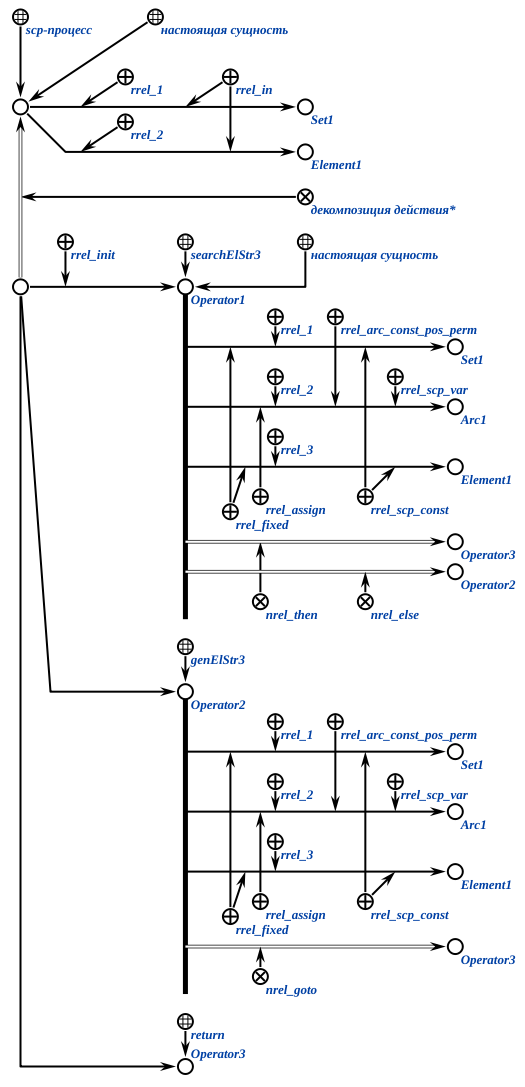
\includegraphics[width=40mm]{figures/sd_sets/process_example.png}
		\end{center}}
\end{frame}

\begin{frame}%пояснение процесса			
			\scntext{пояснение}{Осуществляется вызов \textit{scp-программы}. Генерируется соответствующий \textit{scp-процесс}. Происходит инициирование начального оператора scp-процесса \textit{Operator1}}
\end{frame}

\begin{frame}{\\scp-оператор}%scp-оператор
	\topline
	\justifying
	\begin{SCn}
		\scnheader{scp-оператор}
		\scnrelto{включение}{действие в sc-памяти}
				\scnrelto{семейство подмножеств}{атомарный тип scp-оператора}
				\begin{scnrelfromset}{разбиение}
					\scnitem{scp-оператор генерации конструкций}
					\scnitem{scp-оператор ассоциативного поиска конструкций}
					\scnitem{scp-оператор удаления конструкций}
					\scnitem{scp-оператор проверки условий}
					\scnitem{scp-оператор управления значениями операндов}
					\scnitem{scp-оператор управления scp-процессами}
					\scnitem{scp-оператор управления событиями}
					\scnitem{scp-оператор обработки содержимых файлов}
					\scnitem{scp-оператор управления блокировками}
				\end{scnrelfromset}
	\end{SCn}
	\vspace{-2 em}
\end{frame}

%\begin{frame}%классификация2
%	\begin{SCn}
%		
%		\begin{textitemize}
%			\item{scp-оператор генерации конструкций}
%		\end{textitemize}
%		\begin{scnrelfromset}{разбиение}
%			\scnitem{scp-оператор генерации конструкции по произвольному образцу}
%			\scnitem{scp-оператор генерации одноэлементной конструкции}
%			\scnitem{...}
%		\end{scnrelfromset}
%		
%		\begin{textitemize}
%			\item{scp-оператор ассоциативного поиска конструкций}
%		\end{textitemize}
%		\begin{scnrelfromset}{разбиение}
%			\scnitem{scp-оператор поиска конструкции по произвольному образцу}
%			\scnitem{scp-оператор поиска пятиэлементной конструкции с формированием множеств}
%			\scnitem{scp-оператор поиска трехэлементной конструкции}
%			\scnitem{...}
%		\end{scnrelfromset}
%	\end{SCn}
%\end{frame}
%
%\begin{frame}%классификация3
%	\begin{SCn}	
%		\begin{textitemize}
%			\item{scp-оператор удаления конструкций}
%		\end{textitemize}
%		\begin{scnrelfromset}{разбиение}
%			\scnitem{scp-оператор удаления множества элементов трехэлементной конструкции}
%			\scnitem{scp-оператор удаления пятиэлементной конструкции}
%			\scnitem{...}
%		\end{scnrelfromset}
%		
%		\begin{textitemize}
%			\item{scp-оператор проверки условий}
%		\end{textitemize}
%		\begin{scnrelfromset}{разбиение}
%			\scnitem{scp-оператор сравнения числовых содержимых файлов}
%			\scnitem{scp-оператор проверки равенства числовых содержимых файлов}
%			\scnitem{scp-оператор проверки совпадения значений операндов}
%			\scnitem{scp-оператор проверки наличия содержимого у файла}
%			\scnitem{scp-оператор проверки наличия значения у переменной}
%			\scnitem{scp-оператор проверки типа sc-элемента}
%		\end{scnrelfromset}	
%	\end{SCn}
%\end{frame}
%
%\begin{frame}%классификация4
%	\begin{SCn}
%		
%		\begin{textitemize}
%			\item{scp-оператор управления значениями операндов}
%		\end{textitemize}
%		\begin{scnrelfromset}{разбиение}
%			\scnitem{scp-оператор удаления значения переменной}
%			\scnitem{scp-оператор присваивания значения переменной}
%		\end{scnrelfromset}
%		
%		\begin{textitemize}
%			\item{scp-оператор управления scp-процессами}
%		\end{textitemize}
%		\begin{scnrelfromset}{разбиение}
%			\scnitem{scp-оператор удаления значения переменной}
%			\scnitem{scp-оператор завершения выполнения программы}
%			\scnitem{конъюнкция предшествующих scp-операторов}
%			\scnitem{scp-оператор ожидания завершения выполнения scp-программы}
%			\scnitem{...}
%		\end{scnrelfromset}	
%		\begin{textitemize}
%			\item{scp-оператор управления событиями}
%		\end{textitemize}
%		\scnsuperset{scp-оператор ожидания события}
%	\end{SCn}
%\end{frame}
%
%\begin{frame}%классификация5
%	\begin{SCn}
%		\begin{textitemize}
%			\item{scp-оператор обработки содержимых файлов}
%		\end{textitemize}
%		\begin{scnrelfromset}{разбиение}
%			\scnitem{scp-оператор вычисления арксинуса числового содержимого файла}
%			\scnitem{scp-оператор деления числовых содержимых файлов}
%			\scnitem{scp-оператор вычисления логарифма числового содержимого файла}
%			\scnitem{scp-оператор удаления содержимого файла}
%			\scnitem{scp-оператор копирования содержимого файла}
%			\scnitem{scp-оператор нахождения остатка от деления числовых содержимых файлов}
%			\scnitem{scp-оператор перевода в верхний регистр строкового содержимого файла}
%			\scnitem{scp-оператор получения части строкового содержимого файла по индексам}
%			\scnitem{scp-оператор вычисления длины строкового содержимого файла}
%			\scnitem{scp-оператор разбиения строки на подстроки}
%			\scnitem{...}
%		\end{scnrelfromset}
%	\end{SCn}
%\end{frame}
%
%\begin{frame}%классификация6
%	\begin{SCn}
%		\begin{textitemize}
%			\item{scp-оператор управления блокировками}
%		\end{textitemize}
%		\begin{scnrelfromset}{разбиение}
%			\scnitem{scp-оператор снятия всех блокировок данного scp-процесса}
%			\scnitem{cp-оператор установки полной блокировки на sc-элемент}
%			\scnitem{scp-оператор снятия блокировки со структуры}
%			\scnitem{scp-оператор установки блокировки на изменение структуры}
%			\scnitem{...}
%		\end{scnrelfromset}	
%	\end{SCn}
%	
%\end{frame}

\begin{frame}%пояснение оператора
	\begin{SCn}	
		\scntext{пояснение}{Каждый \textbf{\textit{scp-оператор}} представляет собой некоторое элементарное \textit{действие в sc-памяти}. Аргументы \textit{scp-оператора} будем называть операндами. Порядок операндов указывается при помощи соответствующих ролевых отношений (\textit{1\scnrolesign}, \textit{2\scnrolesign}, \textit{3\scnrolesign} и так далее). Операнд, помеченный ролевым отношением \textit{1\scnrolesign}, будем называть первым операндом, помеченный ролевым отношением \textit{2\scnrolesign} – вторым операндом, и т.д. Тип и смысл каждого операнда также уточняется при помощи различных подклассов отношения \textit{scp-операнд\scnrolesign}. В общем случае операндом может быть любой \textit{sc-элемент}, в том числе, знак какой-либо \textit{scp-программы}, в том числе самой программы, содержащей данный оператор.\\
			
			Каждый \textbf{\textit{scp-оператор}} должен иметь один и более операнд, а также указание того \textbf{\textit{scp-оператора}} (или нескольких), который должен быть выполнен следующим. Исключение их данного правила составляет \textit{scp-оператор завершения выполнения программы}, который не содержит ни одного операнда и после выполнения которого никакие \textit{scp-операторы} в рамках данной программы выполняться не могут.}
\end{SCn}
	\end{frame}

\begin{frame}{\\Атомарный тип scp-оператора}%атомарный тип
	\topline
	\justifying
	\begin{SCn}
		\scnheader{атомарный тип scp-оператора}
		\scntext{пояснение}{Каждый \textbf{\textit{атомарный тип scp-оператора}} представляет собой класс \textit{scp-операторов}, который не разбивается на более частные, и, соответственно, интерпретируется реализацией \textit{Aбстрактной scp-машины}. }
		\end{SCn}
\end{frame}

\begin{frame}{\\Начальный scp-оператор}%начальный scp-оператор
	\topline
	\justifying
	\begin{SCn}	
		\scnheader{начальный оператор\scnrolesign}
		\scnsubset{1\scnrolesign}
		\scntext{пояснение}{Ролевое отношение \textbf{\textit{начальный оператор\scnrolesign}} указывает в рамках декомпозиции соответствующего \textit{\mbox{scp-программе}} \textit{scp-процесса} те \textit{scp-операторы}, которые должны быть выполнены в первую очередь, т.е. те, с которых собственно начинается выполнение \textit{scp-процесса}.}
		\end{SCn}
	\end{frame}

\begin{frame}{\\scp-операнд}%scp-операнд разбиение
	\topline
	\justifying
	\begin{SCn}
		\scnheader{scp-операнд\scnrolesign}
		\scnrelto{включение}{аргумент действия\scnrolesign}
		\scniselement{неосновное понятие}
		\scniselement{ролевое отношение}
		\begin{scnrelfromset}{разбиение}
			\scnitem{scp-переменная\scnrolesign}
			\scnitem{scp-константа\scnrolesign}			
			\end{scnrelfromset}
		\begin{scnrelfromset}{разбиение}
			\scnitem{scp-операнд с заданным значением\scnrolesign}
			\scnitem{scp-оперенд со свободным значением\scnrolesign}
		\end{scnrelfromset}
	\begin{scnrelfromset}{разбиение}
		\scnitem{константный sc-элемент\scnrolesign}
		\scnitem{переменный sc-элемент\scnrolesign}
	\end{scnrelfromset}
\end{SCn}
\vspace{-2.3em}
\end{frame}

\begin{frame}%sc-операнд с заданным значением
	\scnheader{scp-операнд с заданным значением\scnrolesign}
	\scntext{пояснение}{Значение операндов, помеченных ролевым отношением \textit{scp-операнд с заданным значением\scnrolesign}, считается заданным в рамках текущего \textit{scp-оператора}. Данное значение учитывается при выполнении \textit{scp-оператора} и остается неизменным после окончания выполнения \textit{scp-оператора}. Каждая \textit{scp-константа\scnrolesign} по умолчанию рассматривается как \textit{scp-операнд с заданным значением\scnrolesign}, в связи с чем явное использование данного ролевого отношения в таком случае является избыточным. В таком случае в качестве значения рассматривается непосредственно сам операнд. В случае если отношением \textit{\mbox{scp-операнд} с заданным значением\scnrolesign} помечена \textit{scp-переменная\scnrolesign}, то осуществляется попытка поиска значения для данной \textit{scp-переменной\scnrolesign} (ее элемента). Если попытка оказалась безуспешной, то возникает ошибка времени выполнения, которая должна быть обработана соответствующим образом.
		
		Любой \textit{scp-операнд с заданным значением\scnrolesign} независимо от конкретного типа \textit{scp-оператора} может быть \textit{scp-переменной\scnrolesign}.}
\end{frame}

\begin{frame}%sc-операнд со свободным значением
	\scnheader{scp-операнд со свободным значением\scnrolesign}
	\scntext{пояснение}{Значение операндов, помеченных ролевым отношением \textit{scp-операнд со свободным значением\scnrolesign}, считается свободным (не заданным заранее) в рамках текущего \textit{scp-оператора}. В начале выполнения \textit{scp-оператора} связь между \textit{scp-переменной\scnrolesign}, помеченной данным ролевым отношением, и ее элементом (значением) всегда удаляется. В результате выполнения данного оператора может быть либо сгенерировано новое значение \textit{scp-переменной\scnrolesign}, либо не сгенерировано, тогда \textit{scp-переменная\scnrolesign} будет считаться не имеющей значения. Ни одна \textit{scp-константа\scnrolesign} не может быть помечена как \textit{scp-операнд со свободным значением\scnrolesign}, поскольку константа не может изменять свое значение в ходе интерпретации \textit{scp-программы}.}
\end{frame}

\begin{frame}%разбиение2
	\begin{SCn}
\begin{scnrelfromlist}{включение}
\scnitem{формируемое множество\scnrolesign}
\begin{scnrelfromset}{разбиение}
	\scnitem{формируемое множество 1\scnrolesign}
	\scnitem{формируемое множество 2\scnrolesign}
	\scnitem{формируемое множество 3\scnrolesign}
	\scnitem{формируемое множество 4\scnrolesign}
	\scnitem{формируемое множество 5\scnrolesign}
	\end{scnrelfromset}
\scnitem{удаляемый sc-элемент\scnrolesign}	
\scnitem{тип sc-элемента\scnrolesign}
		\begin{scnrelfromset}{разбиение}
			\scnitem{sc-узел\scnrolesign}
			\scnitem{sc-дуга\scnrolesign}
			\scnitem{sc-ребро\scnrolesign}
			\scnitem{файл\scnrolesign}
			\end{scnrelfromset}
		\end{scnrelfromlist}
		\end{SCn}
\end{frame}

\begin{frame}%пояснение
	\begin{SCn}
		\scntext{пояснение}{Ролевое отношение \textit{scp-операнд\scnrolesign} является неосновным понятием и указывает на принадлежность аргументов \textit{scp-оператору}. Помимо указания какого-либо класса \textit{scp-операндов\scnrolesign} порядок аргументов \textit{scp-оператора} дополнительно уточняется \textit{ролевыми отношениями 1\scnrolesign}, \textit{2\scnrolesign} и т. д.}
		\end{SCn}
	\end{frame}

\begin{frame}{\\sc- узел}%sc-узел
	\topline
	\justifying
	\begin{SCn}
		\begin{textitemize}
			\item{sc-узел\scnrolesign}
			\end{textitemize}
		\begin{scnrelfromset}{разбиение}
			\scnitem{структура\scnrolesign}
			\scnitem{отношение\scnrolesign}
			\scnrelfrom{включение}{ролевое отношение\scnrolesign}
			\scnitem{класс}
			\end{scnrelfromset}
\end{SCn}
\end{frame}

\begin{frame}{\\sc-дуга}%sc-дуга
	\topline
	\justifying
	\begin{SCn}		
		\begin{textitemize}
			\item{sc-дуга\scnrolesign}
		\end{textitemize}
		\begin{scnrelfromset}{разбиение}
			\scnitem{sc-дуга общего вида\scnrolesign}
			\scnitem{sc-дуга принадлежности\scnrolesign}
			\scnrelfrom{включение}{sc-дуга основного вида\scnrolesign}
			\begin{scnrelfromset}{разбиение}
				\scnitem{позитивная sc-дуга принадлежности\scnrolesign}
				\scnitem{негативная sc-дуга принадлежности\scnrolesign}
				\scnitem{нечеткая sc-дуга принадлежности\scnrolesign}
				\end{scnrelfromset}
			\begin{scnrelfromset}{разбиение}
				\scnitem{временная sc-дуга принадлежности\scnrolesign}
				\scnitem{постоянная sc-дуга принадлежности\scnrolesign}
			\end{scnrelfromset}
		\end{scnrelfromset}
		
	\end{SCn}
\vspace{-3em}
\end{frame}

\begin{frame}{\\sc-переменная}%sc-переменная
	\topline
	\justifying
	\scnheader{scp-переменная\scnrolesign}
	\scntext{пояснение}{В рамках \textit{scp-программы} \textit{scp-переменные\scnrolesign} не обрабатываются явно при интерпретации, обрабатываются значения переменных. Каждая переменная \textit{scp-программы} может иметь одно значение в каждый момент времени, т. е. представляет собой ситуативный \textit{синглетон}, элементом которого является текущее значение \textit{scp-переменной\scnrolesign}. Значение каждой \textit{scp-переменной\scnrolesign} может меняться в ходе интерпретации \textit{scp-программы}. При этом интерпретатор при обработке \textit{scp-оператора} работает непосредственно со значениями \textit{\mbox{scp-переменных\scnrolesign}}, а не самими \textit{scp-переменными\scnrolesign} (которые также являются узлами той же семантической сети).}
\end{frame}

\begin{frame}{\\sc-константа}%sc-константа
	\topline
	\justifying
	\scnheader{scp-константа\scnrolesign}
	\scntext{пояснение}{В рамках \textit{scp-программы} \textit{scp-константы\scnrolesign} явно участвуют в \textit{\mbox{scp-операторах}} в качестве элементов (в теоретико-множественном смысле) и напрямую обрабатываются при интерпретации \textit{scp-программы}. Константами в рамках \textit{scp-программы} могут быть \textit{sc-элементы} любого типа, как \textit{\mbox{sc-константы}}, так и \textit{\mbox{sc-переменные}}. Константа в рамках \textit{scp-программы} остается неизменной в течение всего срока интерпретации. Константа \textit{\mbox{scp-программы}} может быть рассмотрена как переменная, значение которой совпадает с самой переменной в каждый момент времени, и изменено быть не может. Таким образом, далее будем считать, что \textit{scp-константа\scnrolesign} и ее значение это одно и то же. Каждый \textit{in-параметр\scnrolesign} при интерпретации каждой конкретной копии \textit{scp-программы} становится \textit{scp-константой\scnrolesign} в рамках всех ее операторов, хотя в исходном теле данной программы в каждом из этих операторов он является \textit{scp-переменной\scnrolesign}.}
\vspace{-2em}	
\end{frame}

\begin{frame}{\\агентная scp-программа}%агентная scp-программа
	\topline
	\justifying
	\scnheader{агентная scp-программа}
	\scnsubset{scp-программа}
	\scntext{пояснение}{\textit{Scp-программы} данного класса представляют собой реализации программ агентов обработки знаний, и имеют жестко фиксированный набор параметров. Каждая такая программа имеет ровно два \textit{in-параметра\scnrolesign}. Значение первого параметра является знаком бинарной ориентированной пары, являющейся вторым компонентом связки отношения \textit{первичное условие инициирования*} для абстрактного \textit{sc-агента}, в множество \textit{программ sc-агента*} которого входит рассматриваемая \textbf{\textit{агентная scp-программа}}, и, по сути, описывает класс событий, на которые реагирует указанный sc-агент.
		
		Значением второго параметра является \textit{sc-элемент}, с которым непосредственно связано событие, в результате возникновения которого был инициирован соответствующий \textit{sc-агент}, т.е., например, сгенерированная либо удаляемая \textit{sc-дуга} или \textit{sc-ребро}.}
	\vspace{-2em}
	\end{frame}
